\documentclass[11pt]{article}
\usepackage{appendix}
\usepackage{graphicx} 
\usepackage{setspace}
\usepackage{amsmath,float,verbatim,multicol}
\usepackage{array}
\usepackage{lscape}
\usepackage{hyperref}

\usepackage{amssymb}
\bibliographystyle{plainnat}
\usepackage[round]{natbib}
\usepackage{multirow}
\usepackage{xcolor}

\setlength{\textheight}{8.8in} \setlength{\textwidth}{6.3in}
\setlength{\oddsidemargin}{0.2in} \setlength{\topmargin}{-0.30in}
\setlength{\footnotesep}{10.0pt}

\newcommand{\ol}{\overline}



\renewcommand{\baselinestretch}{1.25}
\title{Solving a McCall Search Model via Reinforcement Learning}
\author{ Trevor Gallen \\ Econ 64200 }
\date{Fall 2022}

\begin{document}
\bibliographystyle{myplainnat}
%\bibpunct{(}{)}{;}{a}{}{,}6868

\maketitle


\textbf{Deliverables}
\begin{itemize}
\item You should have a word/\LaTeX document that has three sections: 
\begin{enumerate}
\item Discusses the model and answers the questions I pose throughout.
\item Contains the tables and figures you will produce.
\item Contains a discussion of your programming choices if you had to make any.
\end{enumerate}
\item You should have a Matlab file or set of files (zipped) that contain \textbf{all} your programs and raw data.  There should be a file called ``Main.M" that produces everything I need in one click.
\end{itemize}
\ \\
\ \\


\section{Model}
In this homework, we're going to try to solve a simple McCall search model with Reinforcement Learning.  \\
\ \\
Each period, agents wage up with a wage draw  $w\sim\log\mathcal{N}\left(1,3\right)$, they have a choice whether or not to accept the offer or not.  If they accept, they receive that $w^{accepted}$ draw every period for the rest of their life.  If they reject, then (if they don't die) receive zero and get a new wage draw in the next period, discounted by a factor of $\beta$.  The probability of death is $\alpha=0.067$, discount factor is $\beta=0.95$.  Their problem is can therefore be written:

$$V(w)=\underset{accept,reject}{\max}\left\{\frac{w}{1-(1-\alpha)\beta},(1-\alpha)\beta V(w')\right\}$$

\section{Problem}
Set this problem up and solve it with a reinforcement learning agent in Matlab.  Note that while the state is continuous, the decision is discrete.  However, you may make a discrete decision continuous (round a sigmoid function, for instance), and approximate a continuous state with a discrete set of $N$ levels.  To solve this, you must therefore:
\begin{enumerate}
\item Set up an action space (accept/reject) and observation space (wage draw)
\item Set up neural networks (if actor critic, then a critic network that takes in one action and one state and spits out a scalar, and an action network that takes in a state and spits out an action)
\item Set up a reset function that starts your actor
\item Set up a step function that advances them one period, or terminates the problem if they accept (or die)
\end{enumerate}
This can be as simple as creating the observation info (rlNumericSpec(dimensions)), the act info (rlFiniteSetSpec(discrete actions), set up the environment (rlFunctionEnv(obsInfo,actInfo,stepfcn,resetfcn)) and then setting up a default DQN agent (rlDQNAgent(obsInfo,actInfo)), telling it the discount factor (agent.AgentOptions.DiscountFactor = xxx), and training it train(agent,env,opt).  \textbf{I leave it to you} how you solve it, this is merely a suggestion.\\
 Once you've solved the problem, you should graph out:
 \begin{itemize}
 \item The value function of each action, contingent on draw (getValue(getCritic(agent,wage draw)))
 \item The action at each wage draw getAction(agent,wage draw)
 \end{itemize}
 \ \\
 \ \\
 \textbf{Suggested Solution}\ \\
 \ \\
 The simplest way to do this is to take Matlab's default Neural Networks.  I choose to use a DQN agent, a ``deep Q-network"  agent.  This agent is a little different than our actor-critic agents, it focuses on the ``critic" part, and has a deep neural network to approximate it.  The basic idea is the same, however--if tries to learn the Q-function (value of state+action) rather than the value-function (value of state, assuming action maximizes).  It does so by starting out with an NN that takes in a state action pair, selects either a random action (exploration) or what it thinks is best (greedy), and stores the experience.  After doing so multiple times, it has a dataset of state-action-rewards/experiences that it can use to update its network.  Maximizing is easy in this case, because actions are discrete.\\
 \ \\
 When I do this, I have three functions:
 \begin{itemize}
 \item Main.m, which:
 \begin{itemize}
 \item Sets up the observation info
 \item Sets up the action info
 \item Defines the environment (observation info, action info, reset function, and step function)
 \item Creates the agent (passes observation \& action info to rlDQNagent)
 \item Trains the agent
 \item What is spit out is a little different than a critic we saw, as evaluating it gives two values (value of accept \& value of reject).
 \item It retrieves \& plots the values, and the actions.
 \end{itemize}
 \item myresetfunction, which:
 \begin{itemize}
 \item Draws one random draw from a lognormal distribution as the state (that's it!)
 \end{itemize}
 \item mystepfunction, which:
 \begin{itemize}
 \item Pulls in the action \& the state
 \item Determines if you die this period (draws a draw)
 \item If you don't die and accept, then it gives you the NPV reward, tells simulator it's done
 \item If you don't die and reject, then gives you a new draw, tells simulator it isn't done
 \item If you die, then you get no reward, tells simulator it's done
 \end{itemize}
 \end{itemize}
  That's it!  Shockingly easy to read, as opposed to VFI, which can be less easy to read (simulating a single draw is simpler than integration, no need to write a maximization step, no explicit looping over values).  A few interesting lessons:
  \begin{itemize}
  \item We aren't integrating--the program is doing that for us, via monte carlo
  \item However, it's hard to learn about ``rare" events, by their very nature, and lognormal has a lot of rare events!
  \item Consequently it takes time to converge
  \item I let it run for 16,000 trials, and plotted the results below, which aren't insane, but you can see some of the issues:  
  \begin{itemize}
  \item the reject value should be flat (it is, approximately, but not perfect)
  \item the accept value should be linear (it is, approximately, but not perfect)
  \item If you solve for the reservation wage in closed form, with $w^*$ the reservation wage, $\beta$ the discount factor*chance of living, and $F(w)$ the cumulative distribution function for the wage lognormal with mean 1 and variance 3, you get:
  $$w^*=\frac{\beta}{1-\beta}\int_{w^*}^\infty(w-w^*)dF(w)\Rightarrow w^*=1367$$
  \item Which suggests we should have let it run a little longer!
  \end{itemize}
  \end{itemize}
  
  \begin{figure}[ht!]
  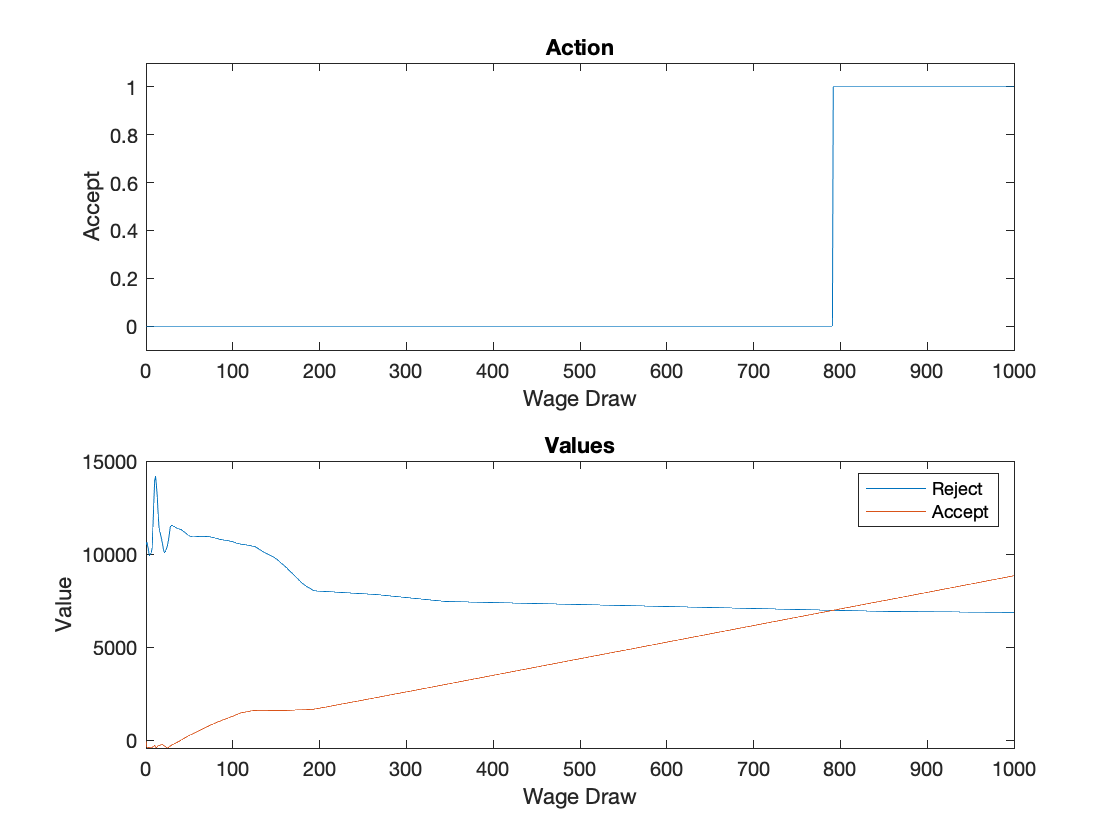
\includegraphics[scale=0.4]{Figure1.png}
  \end{figure}

 \section{Research}
 Change the model in some interesting way and report your results.


\end{document}





